% neginhib cogsci submission


\documentclass[10pt,letterpaper]{article}

\usepackage{cogsci}
\usepackage{pslatex}
\usepackage{apacite}
\usepackage{graphicx}

\title{The development of information processing in three language games}
 
\author{{\large \bf Ann E. Nordmeyer} \\
  \texttt{anordmey@stanford.edu} \\
  Department of Psychology \\
  Stanford University
  \And {\large \bf Erica J. Yoon} \\
  \texttt{ejyoon@stanford.edu} \\
  Department of Psychology \\
  Stanford University
  \And {\large \bf Michael C. Frank} \\
  \texttt{mcfrank@stanford.edu} \\
  Department of Psychology \\
  Stanford University}

\begin{document}

\maketitle


\begin{abstract}

...

\textbf{Keywords:} 
Inhibitory control; negation; implicature; drift diffusion model; cognitive development; pragmatics

\end{abstract}


\section{Introduction}

What happens in a child's mind when they hear a word?  Traditional tests of children's language comprehension often ask a child to respond to words by looking at or pointing to a picture; if the child reliably selects the correct word, then we assume that the child understands the meaning of that word.  Children's performance on even the most simple language comprehension task is typically slower and more error-prone compared to adults, however.  By exploring how children process information in language comprehension tasks, we can clarify our understanding of the many factors at play in children's language processing.

The drift diffusion model \cite<e.g.>{ratcliff1978theory} uses both accuracy and reaction time to model the decision making process in simple two-alternative forced choice paradigms.  The model produces four key parameters: boundary separation (the amount of evidence needed to reach a positive decision), bias (to what extent is the decision process biased towards one decision or another), non-decision time (the time needed to encode basic information about the stimuli, before embarking on the decision process), and drift rate (the rate at which evidence is accumulated).  These parameters capture the decision making process as a noisy accumulation of evidence over time, resulting in an eventual correct or incorrect choice.  Past work has shown that children typically have longer non-decision times, higher separation boundaries, and slower drift rates, suggesting that children require more time to process stimuli, more information to make a decision, and take longer to accumulate evidence compared to adults \cite{ratcliff2012}.  

Exploring how the development of information processing interacts with language comprehension can help us understand why children struggle on certain language tasks.  When a child ``fails'' a challenging language comprehension task, it can be difficult to pinpoint the source of failure; attention demands, memory constraints, or a lack of inhibitory control could all lead children to choose the incorrect picture in response to a word that they know.  For example, even four-year-old children struggle on classic tests of negation comprehension \cite{kim1985, nordmeyer2014b} despite producing negative sentences at a much younger age \cite{bloom1970, pea1980}.  Similarly, children have difficulty processing scalar and ad-hoc implicatures \cite{huang2009, yoonchildren}, despite demonstrating understanding of pragmatic principles from an early age \cite<e.g.>{katsos2011pragmatic, matthews2012tw}.  In both of these examples, children's failures might occur not because they lack linguistic understanding, but because the incorrect choice is more salient or perceptually interesting.  Modeling children's information processing in tasks such as these can help us understand the source of children's difficulty.  

In the current study, we use a simple game with three phases to test adults' and children's inhibitory control, negation comprehension, and implicature comprehension.  We collected both accuracy and reaction time, allowing us to use both traditional analyses and drift diffusion modeling to explore similarities and differences in how adults and children process language across these three tasks.  Despite the fact that the three tasks contained almost identical visual and auditory stimuli, we found distinct patterns of information processing and developmental change across the three games.  We discuss how these results shed light on the development of linguistic processing across early childhood.

\section{Method}

\subsection{Participants}

We invited children the Children's Discovery Museum in San Jose, CA, to play a game to find things that are named.  4-, 5-, and 6-year-olds played the game on a computer (N = FIXME respectively; M = FIXME respectively). (FIXME: exclusion criteria?) We also recruited adult participants (N = FIXME) on Amazon Mechanical Turk to play the computer version of the task.  

\subsection{Stimuli and Design}

AEN.NOTE: I think we should introduce "target" vs. "control" conditions here (i.e. what we mean by that in each game) so that we can use these terms in the results section.

The game consisted of three phases that each tested one of the target processes: inhibition, negation processing, and implicature processing. In each trial in all three phases, there were two images side-by-side on the screen. a Pre-recorded voice said one or two words to refer to the target image, and participants' task was to select the correct referent as soon as they could identify it.

For the ``inhibition'' phase, in a set of 6-8 trials, the same two pictures appeared together (e.g., a picture of a carrot and a picture of a banana), with randomized sides. For the first 5-7 trials ({\emph control}), the same object was named (e.g., ``carrot''), then on the last trial  ({\emph inhibition}), the other object was named (``banana''). Participants were predicted to gain speed on every trial until the last one, in which the accuracy rate was expected to fall, due to the inhibitory demand. Child participants saw a total of 12 sets of trials, and adults saw 24 sets, in the inhibition phase.

For the ``negation'' phase, the referents were named with or without negation. For example, given two pictures of carrot and banana respectively, to refer to the banana the recorded voice said ``banana'' (in a {\emph positive} trial) or ``no carrot'' (in a {\emph negative} trial). Children saw 60 trials, and adults saw 120 trials in the negation phase. 

For the ``implicature'' phase, in each trial there was a picture with one object (e.g., carrot) and another picture with the same object and another one (e.g., carrot and banana). In an {\emph unambiguous} trial, the unique object was named (``banana'') and in an {\emph implicature} trial, the common object was named (``carrot''), implying ``carrot {\emph but not banana''}. Children saw 60 trials, and adults saw 120 trials in the implicature phase. 

\subsection{Procedure}

Adult participants first went through two practice trials, where they were asked to select an obvious, unambiguous referent (e.g., ``cow'' as opposed to ``rabbit''). Then they went through the three test phases in a randomized order.

For child participants, an experimenter first explained the game. Then, for those participants playing the computer version, it proceeded in the same way as for adult participants. For participants playing the iPad version, they played a dots game, where they tapped five dots in random locations, which helped them practice using the iPad screen. Once participants were used to using the screen, they proceeded to the test phases. After the child participants were finished, the experimenter gave them a sticker as a gift and thanked them for playing the game.

\section{Results and Discussion}
AEN.NOTE: do you think we need to talk about traditional RT analyses too?  They're just so boring/unclear for these data so I'm inclined to skip this, but it might seem like a gap.  Maybe we could very briefly discuss RT and accuracy differences (or lack thereof) in the adult data, without showing any plots (just means), and then move on to the DDM analysis for adults and kids.  I'm worried we don't have enough space to include rt/accuracy plots.

AEN.NOTE: I need to go back through and get terminology consistent (e.g. condition vs. trial type).  Also, I should probably refer to the parameters using their conventional symbols, but I've just referred to them by name here.  

We fit the diffusion model separately to each individual participant's data using the RWiener pakage\footnote{All analyses described in this paper were conducted using R version 3.2.1}, which uses the Nelder-Mead method to estimate optimal parameter values.  We estimated parameters separately for each condition (target vs. control) within each game, and calculated the mean and 95\% C.I. across all participants within each age group (4-year-olds, 5-year-olds, 6-year-olds, and adults).  We then used these parameter estimates to produce visualizations of the average decision process for each condition across each game and age group (see Figures \ref{fig:adults} and \ref{fig:kids}).  

\begin{figure}
\begin{center} 
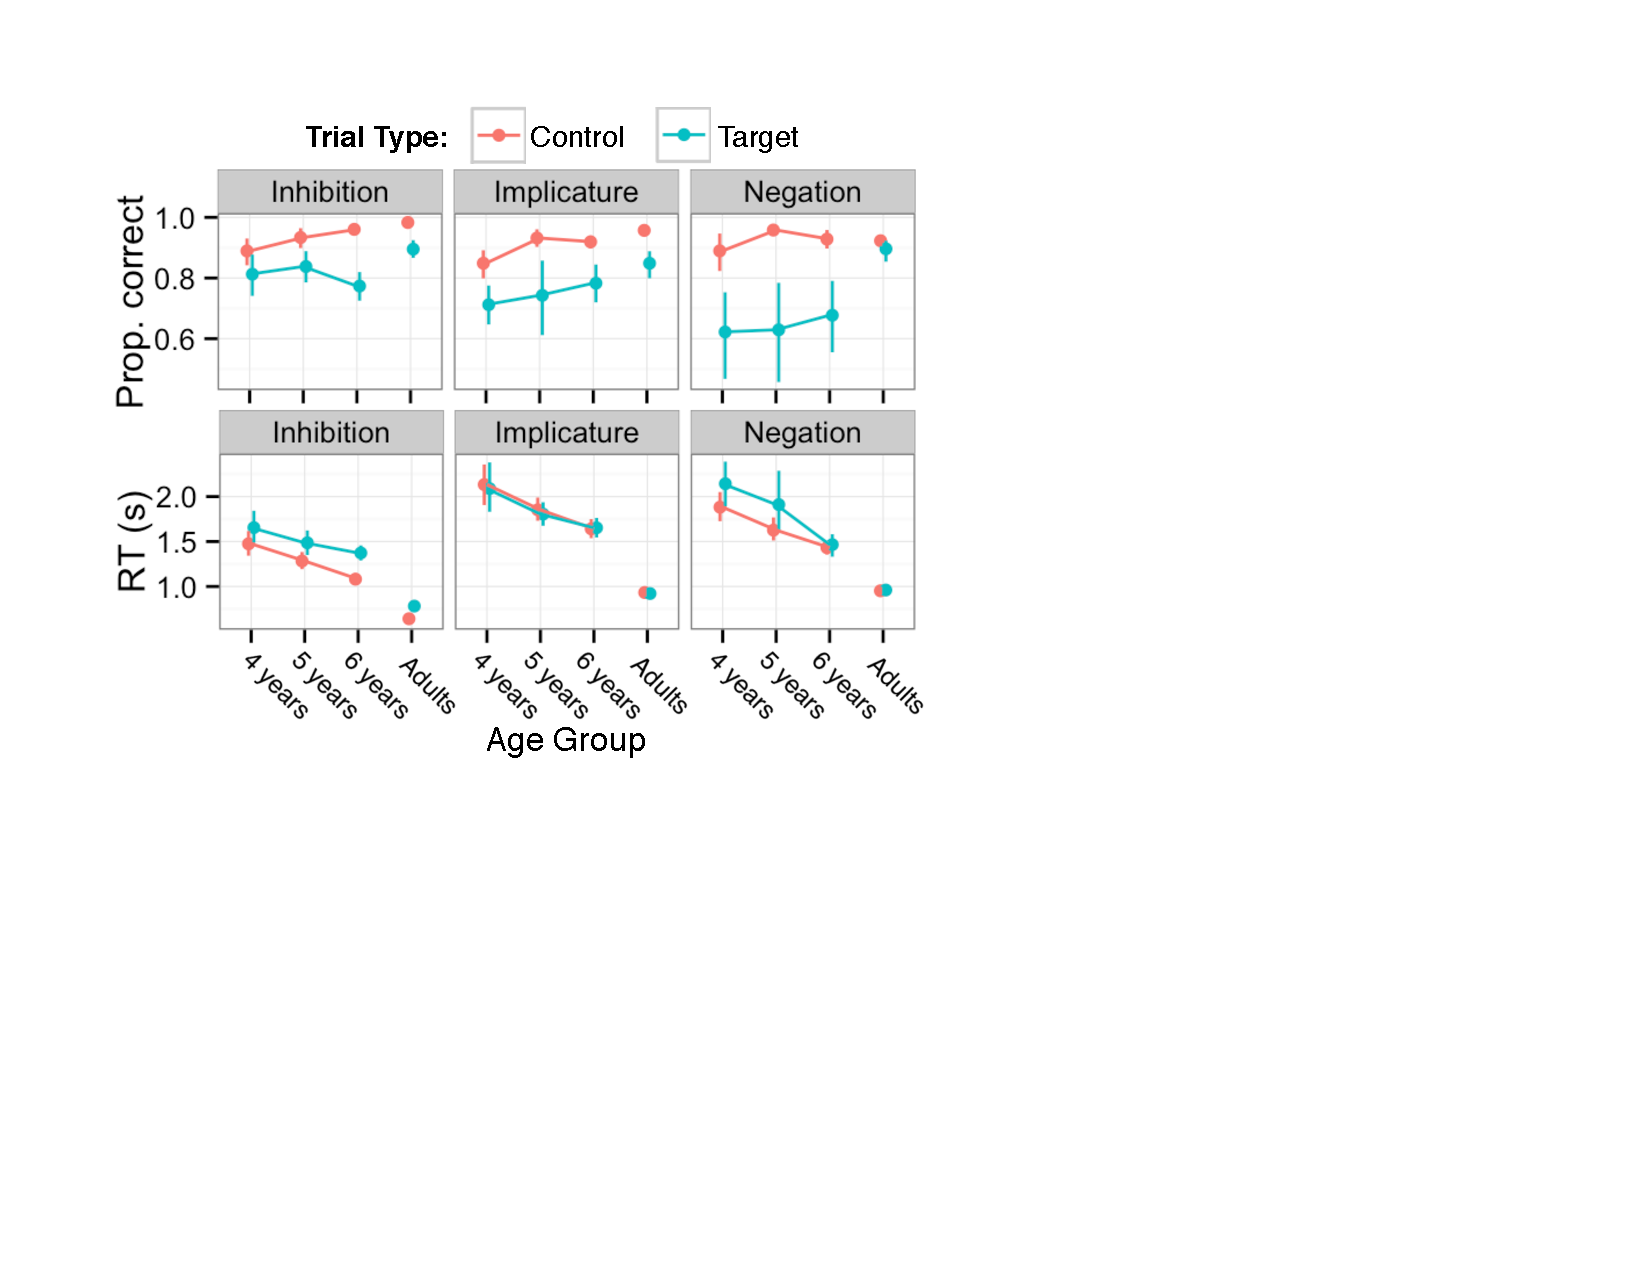
\includegraphics[width=3in]{figures/correct_RT.pdf}
\caption{\label{fig:traditional} DESCRIPTION HERE..}
\end{center} 
\end{figure}

\subsection{Differences across games}

\begin{figure*}
\begin{center} 
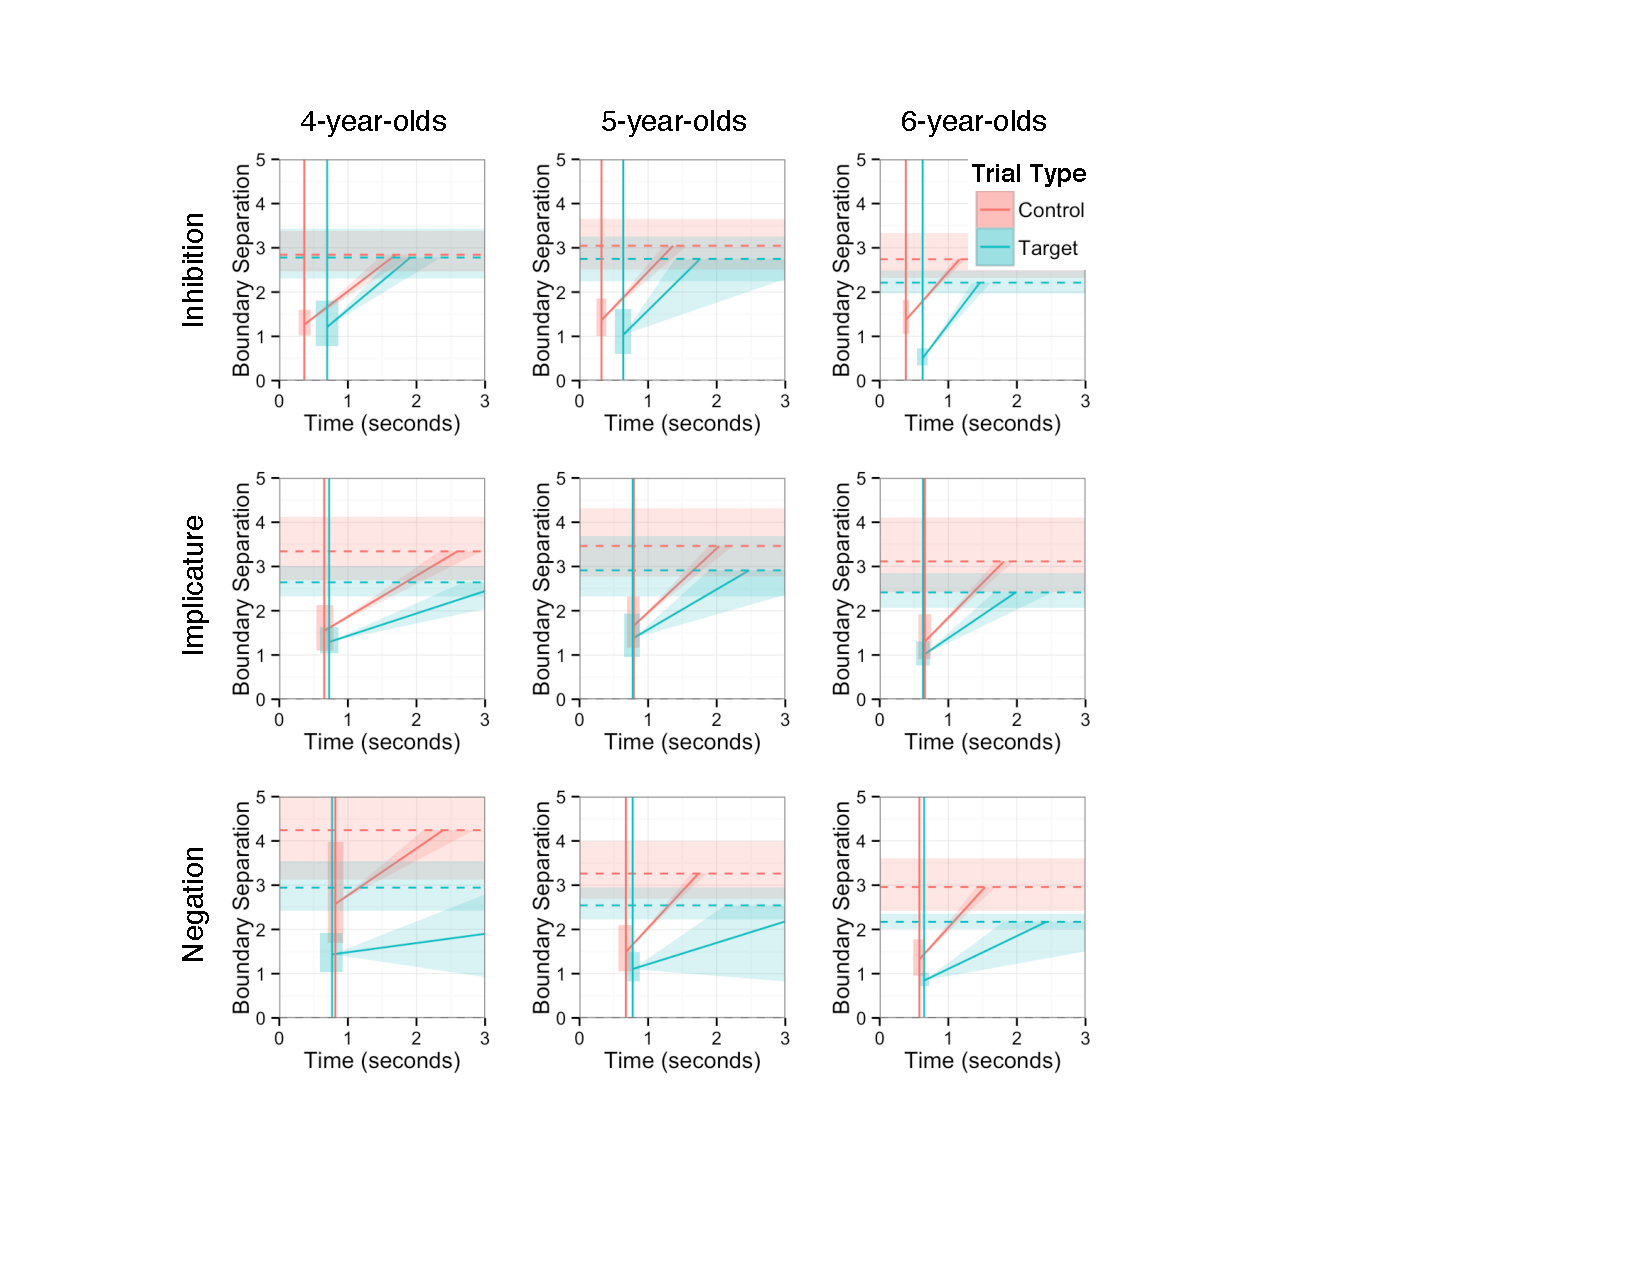
\includegraphics[width=6in]{figures/adult_vis.pdf}
\caption{\label{fig:adults} Visualization of the drift diffusion process for adults across the three games.  The process for control trials is shown in pink, and the process for target trials is shown in green.  The dotted black line at zero represents the threshold for making an incorrect decision, and horizontal colored lines represent the boundary separation parameter (i.e. the threshold for making a correct decision).  Vertical colored lines represent the non-decision time parameter, and the slope of the decision process (angled line) represents the drift rate parameters.  The point where the decision process intercepts the non-decision line represents the bias $\times$ boundary separation.  Ribbons around all lines represent 95\% confidence intervals around each parameter.}
\end{center} 
\end{figure*}

First we explored similarities and differences in the decision process for adults across each of the three games.  We hypothesized that there might be similar process for these three games, because the target trials for each game involve selecting an image that is less salient or interesting for participants.  In Figure 1, we plot the decision process for each of these three games.  Surprisingly, despite the surface similarities of these games, the decision process for control vs. target trials appears to be different across the three games.  In the inhibition game, the most striking difference between control and target (inhibition) trials is the bias towards incorrect trials on target trials.  In the implicatures game, the most striking difference between control (unambiguous) and target (implicature) trials is the higher boundary separation but faster drift rate for control trials compared to target trials.  In the negation game, there appears to be little difference in the decision process between control (positive) and target (negative) trials.

We conducted post-hoc paired t-tests to compare parameter values for control vs. target trials in each game.  In the inhibition game, the bias parameter was significantly lower (e.g. biased towards the incorrect trial) for target trials compared to control trials ($t(47) = 5.05$, $p< .001$).  In the implicature game, the boundary separation and the drift rate were significantly higher for control trials compared to target trials (Boundary Separation: $t(47) = 2.39$, $p< .05$; Drift: $t(47) = 7.35$, $p< .001$).  For the negation game, there was no significant difference between drift rate for control vs. target trials ($t(47) = 1.18$, $p = .24$).  

Although we were surprised by the striking differences across the three games, the decision process that we do see makes sense within the context of each game.  For example, we would expect target trials in the inhibition game to be biased towards incorrect trials, because the game is intentionally designed to create such a bias.  Similarly, the slower drift rate for target trials in the implicatures game makes sense, because these trials are ambiguous (either picture is technically correct), so participants take longer to accumulate enough information to resolve this ambiguity.  The most surprising finding was the lack of difference between positive and negative trials in the negation game.  Past work suggests that adults take longer to respond to negative sentences compared to positive ones \cite{hclark1972}, especially in context-free tasks such as this \cite{nordmeyer2014a}.  One possibility is that the high number of repeated trials, or the simplistic and child-friendly stimuli, made this task easier for adults.

\subsection{Developmental change}

\begin{figure*}
\begin{center} 
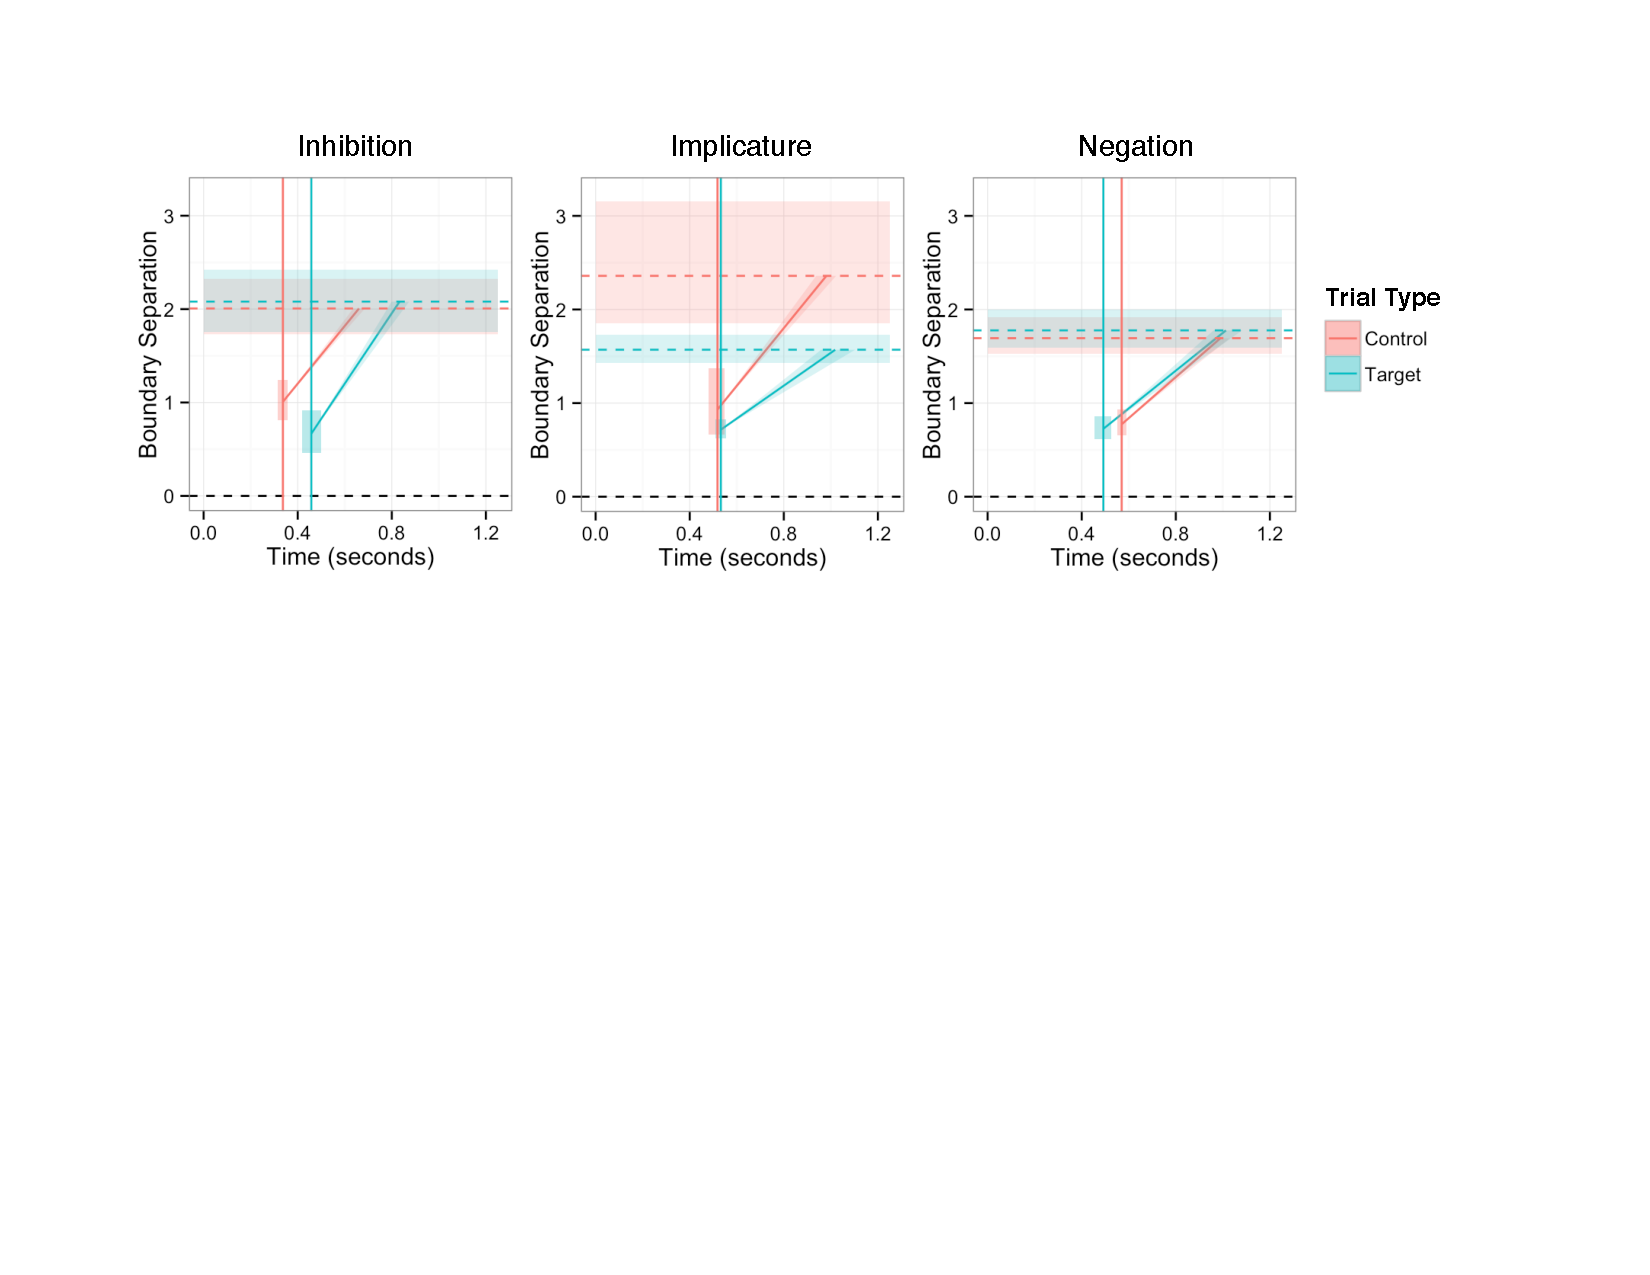
\includegraphics[width=6in]{figures/child_vis.pdf}
\caption{\label{fig:kids} Visualization of the drift diffusion process for 4-year-olds, 5-year-olds, and 6-year-olds across the three games.  Plotting conventions are the same as in Figure \ref{fig:adults}.}
\end{center} 
\end{figure*}

Next we explored developmental change in preschoolers between 4 and 7 years of age.  The decision process for each game across the three age groups is visualized in Figure \ref{fig:kids}.  For the inhibition and implicature games, children at all ages look similar to adults, with developmental change across the three age groups as children's decision process gets more adult-like.  For example, in the inhibition game, 4-year-olds are actually \emph{less} likely to show a bias towards the incorrect trial; this bias appears to get stronger by age 6.  In the implicatures game, children have a slower drift rate for target trials compared to control trials even at age 4, but this difference becomes more striking as children get older.  The most striking difference between children and adults is in the negation game, where the drift rate for target trials is dramatically slower compared to control trials, although developmental change is evident in this game as well.  

To examine the reliability of our findings, we fit linear models to the data for each of the three games to explore how the interaction between condition (control vs. target trials) and age group influences different parameters.  For the bias parameter in the inhibition game, we see a significant interaction between age group and trial type for four-year-olds ($\beta = .17$, $p< .01$) and a marginally significant interaction for five-year-olds ($\beta = .11$, $p = .09$), indicating that for four and five-year-olds the bias parameter for target trials in the inhibition game is higher compared to adults.  There is no interaction between age group and condition for six-year-olds ($\beta = -.09$, $p = .13$), suggesting that six-year-olds are becoming more adult-like in their bias towards the incorrect trial on the inhibition game.

For the drift rate parameter in the implicatures game, we found a main effect of age group, with a significantly slower drift rate overall for four-year-olds ($\beta = -2.16$, $p < .001$), five ($\beta = -1.64$, $p < .001$), and six-year-olds ($\beta = -1.52$, $p < .001$).  There was also a significant interaction between age group and trial type for four-year-olds ($\beta = 0.91$, $p <.01$), fives ($\beta = 0.79$, $p <.05$), and six-year-olds ($\beta = 0.81$, $p <.01$), indicating that the difference between drift rate for target vs. control trials is much smaller for children compared to adults.  We found the opposite pattern in the negation game: Although there was a similar main effect of age group, with children showing significantly slower drift rates overall compared to adults (4-year-olds: $\beta = -1.13$, $p <.001$; 5-year-olds: $\beta = -.52$, $p <.05$; 6-year-olds: $\beta = -.48$, $p <.05$), children at all age groups showed a \emph{greater} difference in drift rate between control and target trials compared to adults, as indicated by significant negative interactions between age group and trial type for all age groups (4-year-olds: $\beta = -.68$, $p <.05$; 5-year-olds: $\beta = -1.02$, $p <.01$; 6-year-olds: $\beta = -.79$, $p <.01$).  

We can also use our data to look at overall changes in the decision process across age groups, regardless of the task that children were engaged in. Across all three games, children at all age groups had higher boundary separation parameters (4-year-olds: $\beta = .98$, $p <.001$; 5-year-olds $\beta = 1.08$, $p <.001$; 6-year-olds: $\beta = .69$, $p <.001$) and longer non-decision times (4-year-olds: $\beta = .17$, $p <.001$; 5-year-olds $\beta = .18$, $p <.001$; 6-year-olds: $\beta = .10$, $p <.001$) compared to adults, suggesting that children take longer to encode information and need more information to make a decision compared to adults.  Children also had significantly slower drift rates compared to adults (4-year-olds: $\beta = -1.46$, $p <.001$; 5-year-olds $\beta = -1.38$, $p <.001$; 6-year-olds: $\beta = -1.17$, $p <.001$), suggesting that children acquire evidence more slowly than adults.  These data replicate past findings from \citeA{ratcliff2012}, which found similar differences between adults and elementary-school aged children, with a much younger sample of children.  

To explore whether these parameters change significantly throughout these early years, we focused just on children's data and analyzed age group as a continuous variable.  This analysis revealed a significant increase in drift rate across these three years ($\beta = .14$, $p < .05$), as well as a marginally significant decrease in non-decision time ($\beta = -.03$, $p = .051$).  These findings indicate that the speed at which children accumulate evidence and the time it takes children to process basic stimuli-level information develops rapidly across early childhood.  

(AEN.NOTE: Are these last two paragraphs worth keeping in?  I think it's a cool extension of the other developmental ddm paper, but it isn't really theoretically relevant to the inhibition stuff).  




\section{Discussion}

%\section{Acknowledgments}
%
%Bing Nursery School, CDM, Stephen Powell, Veronica, Rachel

\bibliographystyle{apacite}

\setlength{\bibleftmargin}{.125in}
\setlength{\bibindent}{-\bibleftmargin}

\bibliography{neginhib}


\end{document}
